%%This is a very basic IEEEtran template.
\documentclass[conference,12pt]{IEEEtran}

\usepackage{setspace}
\usepackage{color}
\usepackage{graphicx}
\usepackage{comment}
\graphicspath{ {images/} }

\setlength{\evensidemargin}{-0.375in}
\setlength{\oddsidemargin} {-0.375in}
\setlength{\textwidth}     {+7.25in}
\setlength{\topmargin}     {+0.00in}
\setlength{\textheight}    {+9.35in}%{+9.25in}
\setlength{\headsep}       {+0.2in}
\setlength{\voffset}       {-0.5in}
\setlength{\headheight}    {+0.00in}


%==============================================================================
%\markboth{}{}
\pagestyle{plain}
%\thispagestyle{plain}
%\doublespacing


%==============================================================================
%==============================================================================



%
\date{April 26, 2016}
\pagenumbering{arabic}

\begin{document}

\title{Study of the Effects of the Black Hole Attack on Mobile Ad-hoc Networks}
\vspace{-0.1in}



\author{
Terrell Blake Turner
\\
Department of Computer Science and Engineering,\\ University of Tennessee at Chattanooga,\\ Chattanooga, TN 37403
\\
%\thanks{
%Acknowledgment The research developed in this paper is supported by . . .
%}
}

%\doublespacing
\maketitle

\section{Introduction}
\label{intro}
A mobile ad hoc network (MANET), is a network that has a collection of mobile hosts with wireless network interfaces that form a temporary network without the aid of any fixed infrastructure or centralized administration. A MANET is referred to as an infrastructure-less network because the mobile nodes in the network dynamically set up paths among themselves to transmit packets \cite{Kale}. This ability can allow the network heal itself if a connection is broken between nodes. Both the use and the development of MANET devices has increased greatly since their implementation. MANETS nodes have the ability to configure themselves without the need of supervision, effectively decreasing the time and cost it takes to deploy them. This ability is also what makes these networks high mobile.

MANETs can be used in a variety of applications all over the world. They have been used by the military as a more robust and reliable form a communication on the digital battlefield. They have been used in sensor networks which allow for remote collection of data such as: temperature, pressure, toxins, and pollutants in different enviroments. Disaster Area Networks can also be set in place in case of destruction of regular communication infrastructure as they can be deployed rapidly \cite{Bakshi}.

Unfortunately, because of the wireless nature of MANETs, new problems and challenges have arisen in their use. Attacks have been made to take advantage of the protocols and behavior of MANETs in order to steal or monitor information, disrupt service, or make unsolicited changes to devices remotely. These attacks go against the confidentiality, integrity, and availability of information, all of which are critical to uphold security of information systems. 

One such attack that can cause issues with the availability of the MANETs is the black hole attack. This attack works by presenting itself as the best gateway to the destination in which a packet is needing to go. A black hole node takes advantage of protocols in this manner and the nearby packets are forwarded to it rather than the legitimate nodes which are actually more efficient. Once the black hole node obtains the packet, it will simply drop it, effectively denying the packet from reaching its destination. This attack can also cause a great deal of performance issues in MANET networks. This paper will discuss these effects to see how much damage they can do to mobile ad hoc networks. 

In section II we will discuss the related work for this paper. Section III will discuss the motivation behind this research followed by the problem statement statement in Section IV. Proposed work, which will discuss the proposed techniques for detecting grey hole attacks, will be discussed in section V. The simulation, which includes the setup, data, and results, will be shown in Section VI. The conclusion will detailed in Sections VII followed by the future scope in section VIII.


\section{Related Work}
Karlof et al \cite{Karlof}, who has been sited in many articles, is considered the first person to detail the various vulnerabilities inside wireless ad hoc networks. This article explains many of the challenges that MANETs face today and provides a solid basis for research opportunities of the attacks. 

Tseng et al \cite{Tseng} have compiled a survey on how the black hole attack works and how it can affect MANETs and the several common protocols used by them. The purpose of the paper was to give a basic overview of the black hole attack for readers. The problem with this paper is that it hinges mostly on theory and does not provide data that can be analyzed to see the effect of the black hole attack objectively.

Dokurer \cite{Dokurer} has tested the effects of the black hole attack on mobile ad hoc networks and has data revealing their negative effects on these types of networks. His work is heavily based upon in this paper as he had provided tools necessary to simulate the black hole attack which have been implemented for this study. Despite the find in his work, he provided little detail in how the black hole attack affects performance of other metrics such as throughput and packet delivery ratio. These lacking metrics will be the essential focus of this paper.

\section{Motivations and contributions}
Mobile ad hoc networks have proven to be very beneficial to its users. They have helped increase mobility, communication, efficiency, entertainment, and gathering of information. Protecting them from attack is necessary to uphold the benefits that we can receive from these information systems. If solutions are not made to prevent such attacks, then the use of MANETs will become more expensive, unreliable, and less secure to use. 

This paper will focus on the black hole attack, one of many attacks that are affecting MANETs today. It is important to analyze the attack to see what potential damage it can cause and how the attack behaves when set up in different environments before an effective solution can be created to detect and mitigate the attack. 

This purpose of this paper is to provide data so that further research can be made on it in the future. This paper is based upon a prior study of the black hole attack, which provided data on the percentage of packets lost by the black hole attack. In order to further the study on the effects of the black hole attack, this paper will also discuss the packet delivery ratio and average bandwidth to help better understand the nature this attack.


\section{The Problem Statement}
The black hole attack, also known as the packet drop attack, is a denial of service attack in which a malicious node on the network broadcast itself as having the shortest distance to the destination of the packet. This can effectively make the other nodes believe that this is true and begin forwarding packets to the malicious node. Once the packet reaches the malicious node, it will drop the packet and any subsequent packets that arrives to it.

These nodes can cause a varying degree of disruption of service depending on their proximity to other nodes and the total number of malicious nodes are present in the network. Even just one well placed malicious node present in the network can actually decrease performance significantly. 

Before detection and prevention measures are implemented into solving the issues of the black and gray hole attacks, it is important to understand the effects that they can have on network performance.  

\section{Proposed Work}
The paper will discuss the effects of they black hole nodes on mobile ad hoc networks using the Ad hoc On-Demand Distance Vector (AODV) protocol. Route Requests (RREQs), Route Replies (RREPs), and Route Errors (RERRs) are the message types defined by AODV. These message types are received via UDP, and normal IP header processing applies\cite{Perkins}. RREQs are sent to valid neighboring nodes to check their distance from the destination node in the network. RREPS messages are given in response to the request which will explain how far that node is from a particular destination. Because of these message, the AODV protocol can actively update itself effervescently. AODV prioritizes the minimum amount of hops when selecting the route for a packet to go. 

The black hole node will take advantage of these messages. Firstly, after receiving a RREQ, it will reply as having a lowest hop count possible to any destination. Since the other nodes are unaware that the black hole node is not a legitimate node, and has the lowest hop count, packets will be directed toward it. Instead of forwarding the packets, the black hole node will drop them. 

Network Simulator 2 (ns2) was used to simulate the environments with three different scenarios each. Firstly, normal functioning networks will be simulated in order to show how a network functions without the presence of malicious nodes. These same scenarios will be used to test the presence of a single malicious node and then again for 5 nodes. Because scenario 1 already has a low amount nodes, only the presence of a single malicious node will be used to test its environment.
The test environment for each of the scenarios are as follows:

\begin{center}
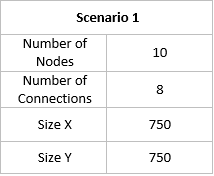
\includegraphics{Scenario1}

Fig 1 - Details of Scenario 1
\linebreak 
\linebreak 
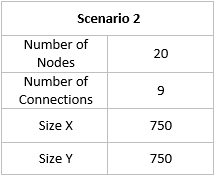
\includegraphics{Scen2}

Fig 2 - Details of Scenario 2
\linebreak 
\linebreak 
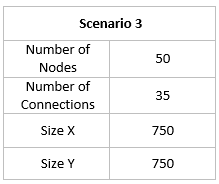
\includegraphics{Scen3}

Fig 3 - Details of Scenario 3
\linebreak 
\end{center}

In order to calculate performance of each of the scenarios, the following metric will be calculated and compared: packets dropped, packet delivery ratio (PDR), and throughput.

In order to calculate the packets dropped, a script will be used to pull the amount of dropped packets from the trace file that is generated after each successful simulation. The script will merely count all the packets dropped on the MAC layer. In environments where at least one malicious node is present, the packets dropped will indicate both packets dropped by the system normally plus the packets dropped by the black hole node. 

In order to calculate the packet delivery ratio, we take the total amount of received packets and subtract them by the amount of packets that have been dropped. Afterwards, the calculated difference is then divide by the total number of packets sent. Mathematically the PDR can be calculated by taking the total packets received divided by the total packets sent, but the reason it is done differently in this study is because the malicious nodes can still receive packets. This means that the trace will actually count the packet as received, even though it will dropped afterwards. This means that the packet will never truly be delivered to the correct node unless the packet is going directly to the black hole node itself.

Throughput will be calculated by taking the packet size of the packets received by legitimate nodes and dividing them by the time frame in which the packets transfer information. Like the calculation of the PDR, if the packet is directed toward a malicious node, it will dropped and not legitimately received by a non-malicious node. Because of this, the packet size of packets received by the malicious node will not be considered when calculating throughput. The result of this calculation will be converted into kilobytes per second (kbps).
\section{Simulation}
To simulate the black hole attack, the AODV protocol needed to copied and altered so that it would function in the same way but drop all packet traffic that goes through it. For this study the blackholeAODV protocol, used in Dokurer's study, will be used to create this effect.

Before implementing the blackholeAODV protocol, the first round of test were for normally functioning networks which do not have any malicious nodes present within them. Second, the same scenarios will be used to test the presence of a single black hole node in the network. Lastly, excluding scenario 1, the scenarios will be be used again to test the effects of 5 black hole nodes in the network. A malicious node will not be added to the environment, but will be exchanged for a legitimate one to maintain the number of nodes allowed in each instance.
\subsection{Data}
\begin{center}
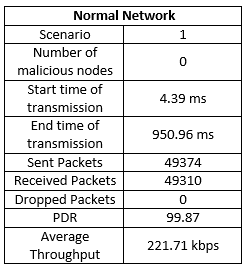
\includegraphics{NNScen1}
\linebreak 
Fig 4 - Details of Normal Environment 1
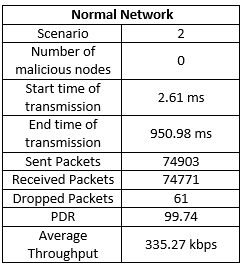
\includegraphics{NNScen2}
\linebreak 
Fig 5 - Details of Normal Environment 2
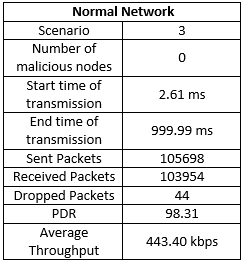
\includegraphics{NNScen3}
\linebreak
Fig 6 - Details of Normal Environment 3
\linebreak 
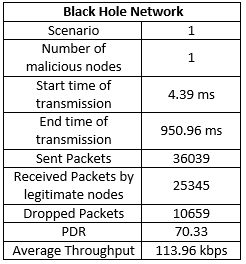
\includegraphics{BHScen1}
\linebreak 
Fig 7 - Details of Attacked Environment 1
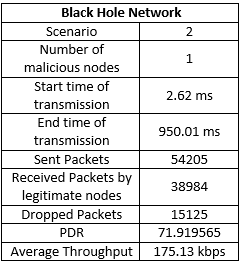
\includegraphics{BHScen2}
\linebreak 
Fig 8 - Details of Attacked Environment 2
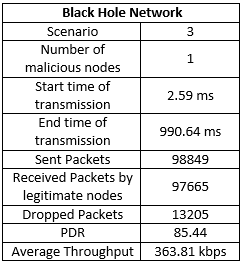
\includegraphics{BHScen3}
\linebreak 
Fig 9 - Details of Attacked Environment 3
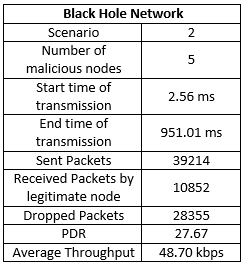
\includegraphics{BH5Scen2}
\linebreak 
Fig 11 - Details of Attacked Environment 4
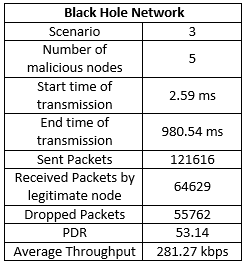
\includegraphics{BH5Scen3}
\linebreak 
Fig 12 - Details of Attacked Environment 5
\end{center}

\subsection{Charts}

\includegraphics{PDChart}
\linebreak 
Fig 13 - Chart of the number of packets dropped

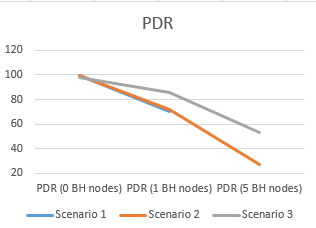
\includegraphics{PDRChart}
\linebreak 
Fig 14 - Chart of the packer delivery ratio

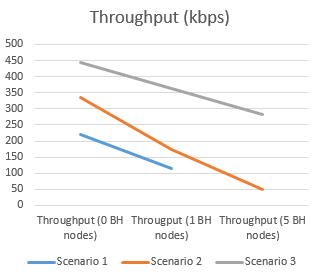
\includegraphics{TPChart}
\linebreak 
Fig 15 - Chart of the average throughput

\subsection{Summary}
The chart in figure 13 shows the total number of packets dropped in each of the environments tested in this study. When no black holes nodes are present in the network, there is very little packet loss and the network performance really efficiently. The highest amount of packet loss in a network with zero malicious nodes was 61 packets. This happens when the Time to Live (TTL) for a packets exceed a certain value and is forced to be dropped. When one malicious node is added to the network, there is a sharp increase in packet drop amount by an average of 12996.33 packets between all the environments. Once 5 black hole nodes were implemented, the graphs varied differently from each other. Scenario 3 has significantly more packets dropped merely because it generated a much greater amount of packets than the other those environments with fewer nodes. 

The chart in figure 14 summarizes the packet delivery ratio of each of the environments. Without any malicious nodes present, the ratio remains very high, never going below 98 percent. With the implementation of a single black hole node, the packet delivery ratio dropped by and average of 24.10 percent across all the networks. Scenario 3 was able to maintain the highest PDR than the other two, which remained about the same. This shows that the increase of legitimate nodes to malicious nodes can still be mitigated by adding more nodes, even if the topography is the same in each scenario. 

The last chart in figure 15 summarizes the average throughput of each scenario. A relationship can be seen between the number of malicious nodes and the performance of the environment. With a single implementation of a black hole node scenario 1 lost 107.75 kbps, scenario 2 lost , and scenario 3 lost. With five black hole nodes implemented: scenario 2 lost 286.57 kbps and scenario 3 lost 162.13 kbps.

\section{Conclusion}
First, the accuracy of these simulations needs to be addressed. Because packet drop is still possible without the presence of a malicious node, some of the calculates may be off by number of 33 drops packets. Despite this small margin of error, the data collected still accurately shows how the black hole node can negatively effect the network. Looking at the comparison of the scenarios from a normally functioning network to the networks with malicious nodes within them, the difference in performance is apparent. In every scenario simulated in this study, the networks with malicious nodes present performed significantly worse than those without them. 

Even with one node present in these network, the average throughput was decreased by at least 14 percent. According to the data obtained from the simulations, a relationship can also be drawn showing that the number of black hole nodes present in the network will lead to a greater decrease in network performance. When there are 5 malicious nodes present, performance is greatly affected. 

In the networks with malicious nodes present, it is observed that increasing the amount of legitimate mobile nodes can actually help mitigate the the effects, but is not an ideal solution to the problem. When comparing figure 9 to figure 8, we can see that the PDR had increased by almost 15 percent, but the amount of nodes is more than double of that detailed in figure 8. The topology size for these scenarios are all the same, thus implying that a large amount of nodes would need to be placed in the same area to get this effect. This is not viable because doubling the amount of nodes can be an expensive and redundant solution to the problem. 
\section{Future Scope}
It is important that data collected for study is as accurate as possible. Some of the data on this paper has a small percentage of error on the calculation of the performance. More controls are needed to ensure that the results of the simulations are more accurate and consistent than what is displayed here. Calculating the performance between communicating nodes instead of the overall performance of the environments could provide helpful data for study as well.

This study covers three similar scenarios using the same area size and assuming that all mobile nodes move within this area. More test can be made in the future to determine if the topology size or a more static placement of nodes to see how they are affected when malicious nodes are introduced to their environments. 

Because of large difference the black hole node creates on the performance metrics of the network, identification of their presence could be made by monitoring the average throughput of the packets and checking if they are consistent to the overall performance of the network before the node was present. This proposed solution has its faults because the performance of the network may be affected by several other factors as well, but interval auditing of the performance can be indication that further investigation should be performed, as long as the investigation is cost effective for the owners of the network. In order to keep MANET nodes inexpensive an easy to deploy, this auditing would have to happen on the protocol level and not by an external monitoring device, in other words, it should remain autonomous. 

Not only do black hole nodes need to be detected, but there needs to be a method for mitigating or eliminating their effects altogether. This would require modifying the AODV protocol itself to give legitimate nodes the ability to recognize the actions carried out by the nodes they share a network with. Once legitimate nodes can identity a faulty or malicious node, they should cease communication with the node to prevent the disruption of service.

Another similar problem to the black hole attack is the gray hole attack. This attack works in the same manor as the black hole attack but can be harder to detect because it will forward packets at specified intervals instead of dropping them altogether. Research into their effects on system performance such as done on the black hole attack in this paper could prove beneficial for future studies. 


%==============================================================================
\begin{thebibliography}{88}
\vspace{-0.02in}


\bibitem{Kale}
Ms.Ruchia A.Kale, Dr. S. R. Gupta.
``AN OVERVIEW OF MANET AD HOC
NETWORK,"
{\em International Journal Of Computer Science And Applications Vol. 6, No.2. Apr 2013.}

\bibitem{Bakshi}
Aditya Bakshi, A.K. Sharma, Atul Mishra.
``Significance of Mobile AD-HOC Networks(MANETS),"
{\em International Journal of Innovative Technology and Exploring Engineering (IJITEE)
ISSN: 2278-3075, Volume-2, Issue-4. March 2013.}

\bibitem{Karlof}
Chris Karlof, David Wagner.
``Secure Routing in Wireless Sensor Networks:
Attacks and Countermeasures,"
{\em Special Issue on Sensor Network Applications and Protocols. Berkeley, California, USA. December 2009.}

\bibitem{Tseng}
Fan-Hsun Tseng, Li-Der Chou, Han-Chieh Chao.
``A survey of black hole attacks in wireless mobile ad hoc networks,"
{\em Human-centric Computing and Information Sciences. 22 November 2011.}

\bibitem{Dokurer}
Drokurer, Semih.
``Black Hole Attack in Wireless Ad-Hoc Networks,"
{\em Atilim University. September 2006.}

\bibitem{Perkins}
C. Perkins, E. Belding-Royer, S. Das.
``Ad hoc On-Demand Distance Vector (AODV) Routing,"
{\em Network Working Group. July 2003.}




%==============================================================================
%==============================================================================
\end{thebibliography}
%\end{spacing}
%==============================================================================
\end{document}


